% For LaTeX-Box: root = stat105_F15_exam1B.tex 
%%%%%%%%%%%%%%%%%%%%%%%%%%%%%%%%%%%%%%%%%%%%%%%%%%%%%%%%%%%%%%%%%%%%%%%%%%%%%%%%
%  File Name: stat105_F15_exam1B.tex
%  Purpose:
%
%  Creation Date: 24-09-2015
%  Last Modified: Thu Oct  1 00:18:21 2015
%  Created By:
%%%%%%%%%%%%%%%%%%%%%%%%%%%%%%%%%%%%%%%%%%%%%%%%%%%%%%%%%%%%%%%%%%%%%%%%%%%%%%%%
\documentclass[addpoints]{examsetup}\usepackage[]{graphicx}\usepackage[]{color}
%% maxwidth is the original width if it is less than linewidth
%% otherwise use linewidth (to make sure the graphics do not exceed the margin)
\makeatletter
\def\maxwidth{ %
  \ifdim\Gin@nat@width>\linewidth
    \linewidth
  \else
    \Gin@nat@width
  \fi
}
\makeatother

\definecolor{fgcolor}{rgb}{0.345, 0.345, 0.345}
\newcommand{\hlnum}[1]{\textcolor[rgb]{0.686,0.059,0.569}{#1}}%
\newcommand{\hlstr}[1]{\textcolor[rgb]{0.192,0.494,0.8}{#1}}%
\newcommand{\hlcom}[1]{\textcolor[rgb]{0.678,0.584,0.686}{\textit{#1}}}%
\newcommand{\hlopt}[1]{\textcolor[rgb]{0,0,0}{#1}}%
\newcommand{\hlstd}[1]{\textcolor[rgb]{0.345,0.345,0.345}{#1}}%
\newcommand{\hlkwa}[1]{\textcolor[rgb]{0.161,0.373,0.58}{\textbf{#1}}}%
\newcommand{\hlkwb}[1]{\textcolor[rgb]{0.69,0.353,0.396}{#1}}%
\newcommand{\hlkwc}[1]{\textcolor[rgb]{0.333,0.667,0.333}{#1}}%
\newcommand{\hlkwd}[1]{\textcolor[rgb]{0.737,0.353,0.396}{\textbf{#1}}}%

\usepackage{framed}
\makeatletter
\newenvironment{kframe}{%
 \def\at@end@of@kframe{}%
 \ifinner\ifhmode%
  \def\at@end@of@kframe{\end{minipage}}%
  \begin{minipage}{\columnwidth}%
 \fi\fi%
 \def\FrameCommand##1{\hskip\@totalleftmargin \hskip-\fboxsep
 \colorbox{shadecolor}{##1}\hskip-\fboxsep
     % There is no \\@totalrightmargin, so:
     \hskip-\linewidth \hskip-\@totalleftmargin \hskip\columnwidth}%
 \MakeFramed {\advance\hsize-\width
   \@totalleftmargin\z@ \linewidth\hsize
   \@setminipage}}%
 {\par\unskip\endMakeFramed%
 \at@end@of@kframe}
\makeatother

\definecolor{shadecolor}{rgb}{.97, .97, .97}
\definecolor{messagecolor}{rgb}{0, 0, 0}
\definecolor{warningcolor}{rgb}{1, 0, 1}
\definecolor{errorcolor}{rgb}{1, 0, 0}
\newenvironment{knitrout}{}{} % an empty environment to be redefined in TeX

\usepackage{alltt}

\usepackage{etoolbox}
\usepackage{tikz,pgfplots}

%% For LaTeX-Box: root = stat105_exam1_info.tex 
%%%%%%%%%%%%%%%%%%%%%%%%%%%%%%%%%%%%%%%%%%%%%%%%%%%%%%%%%%%%%%%%%%%%%%%%%%%%%%%%
%  File Name: stat105_exam1_info.tex
%  Purpose:
%
%  Creation Date: 24-09-2015
%  Last Modified: Thu Sep 24 13:51:36 2015
%  Created By:
%%%%%%%%%%%%%%%%%%%%%%%%%%%%%%%%%%%%%%%%%%%%%%%%%%%%%%%%%%%%%%%%%%%%%%%%%%%%%%%%
\newcommand{\course}[1]{\ifstrempty{#1}{STAT 105}{STAT 105, Section #1}}
\newcommand{\sectionNumber}{B}
\newcommand{\examDate}{October 1, 2015}
\newcommand{\semester}{FALL 2015}
\newcommand{\examNumber}{II}

\newcommand{\examTitle}{Exam \examNumber}

\runningheader{\course{\sectionNumber}}{Exam \examNumber}{\examDate}
\runningfooter{}{}{Page \thepage of \numpages}

\newcommand{\examCoverPage}{
   \begin{coverpages}
   \centering
   {\bfseries\scshape\Huge Exam I \par}
   \vspace{1cm}
   {\bfseries\scshape\LARGE \course{\sectionNumber} \par}
   {\bfseries\scshape\LARGE \semester \par}

   \vspace{2cm}

   \fbox{\fbox{\parbox{5.5in}{\centering 

      \vspace{.25cm} 
      
      {\bfseries\Large Instructions} \\

      \vspace{.5cm} 

      \begin{itemize}
         \item  The exam is scheduled for 80 minutes, from 8:00 to 9:20 AM. At 9:20 AM the exam will end.\\
         \item  A forumula sheet is attached to the end of the exam. Feel free to tear it off.\\
         \item  You may use a calculator during this exam.\\
         \item  Answer the questions in the space provided. If you run out of room, continue on the back of the page. \\
         \item  If you have any questions about, or need clarification on the meaning of an item on this exam, please ask your instructor. No other form of external help is permitted attempting to receive help or provide help to others will be considered cheating.\\
         \item  {\bfseries Do not cheat on this exam.} Academic integrity demands an honest and fair testing environment. Cheating will not be tolerated and will result in an immediate score of 0 on the exam and an incident report will be submitted to the dean's office.\\
      \end{itemize}

   }}}

   \vspace{2cm}

   \makebox[0.6\textwidth]{Name:\enspace\hrulefill}

   \vspace{1cm}

   \makebox[0.6\textwidth]{Student ID:\enspace\hrulefill}
   \end{coverpages}

}


\newcommand{\course}[1]{\ifstrempty{#1}{STAT 105}{STAT 105, Section #1}}
\newcommand{\sectionNumber}{B}
\newcommand{\examDate}{October 1, 2015}
\newcommand{\semester}{FALL 2015}
\newcommand{\examNumber}{I}

%%%%%%%%%%%%%%%%%%%%%%%%%%%%%%%%%%%%%%%%%%%%%%%%%%%%%%%%%%%%%%%%%%%%%%%%%%%%%%%%
\IfFileExists{upquote.sty}{\usepackage{upquote}}{}
\begin{document}

%-- : R code (Code in Document)



\examCoverPage

\begin{questions}

\question

%-- question1: R code (Code in Document)


Two simple tools are used to measure the speed of an object (in meters per second). 
By design and after careful callibration, the true speed of the object is \textit{known} to be 10.4 km/s.
The measurements of the two tools are below: 

\begin{itemize}

   \item Measurements from Tool 1: $ 12.2, 12, 11.7, 11.3, 8.2 $ \\

   \item Measurements from Tool 2: $ 7.4, 7.4, 7.3, 7.4, 7.4 $ \\

\end{itemize}


\begin{parts}
   \part[2] Which tool is better described as accurate?

   \vspace{1cm}

   \part[2] Which tool is better described as precise?

   \vspace{1cm}

\end{parts}

\vspace{1cm}

\question 
%-- functionsAndDatasets: R code (Code in Document)

A sample of size 6 was drawn from a population and the resulting observations are reported below. 
$$
   22, 29, 26, 27, 19
$$
Using these observed values, report the following:

\vspace{1cm}

\begin{parts}

   \part[2] the mean  
   \vspace{2cm}

   \part[2] the variance 
   \vspace{2cm}

   \part[2] the standard deviation 
   \vspace{2cm}

   \part[2] the value of $Q(.25)$
   \vspace{2cm}

\end{parts}

\newpage

\question
Since it is reasonably quick and cost effecient, the complex paints used to line roads, like many liquids, are routinely shipped by train in tanker cars.
However, once the cars arrive at their destination, they often sit for long periods of time before being released to the client - in the case of paint, this waiting time can cause the different components to separate into layers and the paint must be "remixed" before it can be used.
A certain city receives shipments of these paints where they are held at the shipping station for a day before being released.
A civil engineer working for the city plans to test the effectiveness of 5 methods of remixing the paint.
However, there is a small issue: since the tanks themselves are coming from different destinations and through different routes, it is suspected that remixing effectiveness will vary from tank to tank.

Four tanks of paint are currently being shipped. The engineer devises the following plan:

\begin{itemize}
   \item The content of each tank will be divided into 10 parts.
   \item Each part will be randomly assigned an ID from 1 - 10.
   \item Method 1 will be applied to ID 1 and 2, Method 2 will be applied to ID 3 and 4, Method 3 will be applied to ID 5 and 6, Method 4 will be applied to ID 7 and 8, Method 5 will be applied to ID 9 and 10.
\end{itemize}

The city plans to use the method that most effectively separates the paint in the future.


\begin{parts}
   \part[2] Is this an experiment or an observational study? Explain.

  \vspace{2cm}

   \part Identify the following (if there was not one, simply put "not used").

  \vspace{1cm}

   \begin{subparts}
      \subpart[2] Response variable(s):

      \vspace{2cm}

      \subpart[2] Experimental variable(s):

      \vspace{2cm}

      \subpart[2] Blocking variable(s):

      \vspace{2cm}

   \end{subparts}

   \part[2] Was replication used in this experiment? If so, where was it applied? If not, how could we have applied it?

  \vspace{2cm}

\end{parts}

\pagebreak

\question

New Orleans recently made training and use of body cameras mandatory for police officers.
In an \textbf{attempt to determine the effectiveness of the change in policy at reducing the number of accusations of police brutality}, 
a journalist gathered the a week's worth of arrest reports both two months before the policy went into effect and two months after the policy went into effect. 
For each arrest report, she made note of
whether or not the officer was using a body camera,
the time of day (measured in hours so that 1:30 pm is 13.5),
the difficulty reported in the arrest ("suspect resisted with violence", "suspect resisted without violence", or "suspect did not resist"),
and
whether or not the suspect made an accusation of brutality after the arrest.

\begin{parts}
   \part[2] Is this an experiment or an observational study?

   \vspace{2cm}

   \part[2] Identify the response variable(s).

   \vspace{2cm}

   \part For each of the following variables, 

      \begin{itemize}

         \item Identify whether it is qualitative or quantitative variable, and 

         \item If it is qualitative, what are the possible values it can take? If it is quantitative, is it continuous or discrete?

      \end{itemize}

   \begin{subparts}

      \subpart whether or not the office was using a body camera,

      \vspace{2cm}

      \subpart the time of day

      \vspace{2cm}

      \subpart The amount of resistance to arrest

      \vspace{2cm}

      \subpart whether or not the suspect made an accusation of brutality after the arrest

      \vspace{2cm}

   \end{subparts}

\end{parts}
\pagebreak

\question 

%-- : R code (Code in Document)


A certain make of load bearing beam used in construction of large buildings is certified to withstand pressures of 2.5 tonnes per square inch.
30 beams were tested and the pressures at which they failed are collected in the table below.

%-- : R code (Code in Document)
\begin{knitrout}
\definecolor{shadecolor}{rgb}{0.969, 0.969, 0.969}\color{fgcolor}\begin{kframe}
\begin{verbatim}

  The decimal point is at the |

  1 | 2
  2 | 4
  3 | 7
  4 | 345555677888899
  5 | 0012234456
  6 | 35
\end{verbatim}
\end{kframe}
\end{knitrout}

Note that \verb!0 | 9! represents 0.9. In this case, the first quartile is $Q(.25) = 4.5$, 
the median is 4.8, and the third quartile is $Q(.75) = 5.2$.

\begin{parts}
  \part[10] Complete the following frequency table: \\

  \begin{table}[h!]
     \centering
     \begin{tabular}{|l|p{3cm}|p{3cm}|p{4cm}|}
        \hline
                             & \textbf{Frequency} & \textbf{Relative} & \textbf{Cumulative}  \\
        \textbf{Value Range} &                    & \textbf{Frequency} & \textbf{Relative Frequency} \\\hline \hline
                    &  &  &  \\
      0.00 - 2.00   &  &  &  \\
                    &  &  &  \\ \hline
                    &  &  &  \\
      2.01 - 4.00   &  &  &  \\
                    &  &  &  \\ \hline
                    &  &  &  \\
      4.01 - 6.00   &  &  &  \\
                    &  &  &  \\ \hline
                    &  &  &  \\
      6.01 - 8.00   &  &  &  \\
                    &  &  &  \\ \hline
     \end{tabular}
  \end{table}

  \part[10] Using the axes below, create a box plot to summarize the data. Carefully label the axes.

%-- : R plot (results in document)
\begin{knitrout}
\definecolor{shadecolor}{rgb}{0.969, 0.969, 0.969}\color{fgcolor}
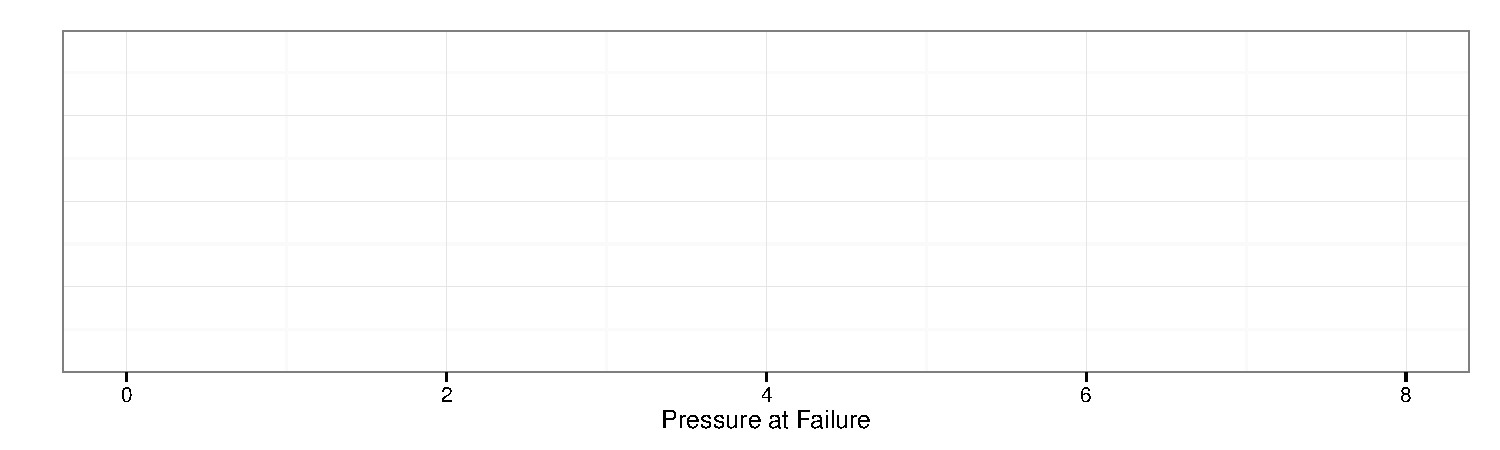
\includegraphics[width=.9\linewidth]{figure/unnamed-chunk-4-1} 

\end{knitrout}

\newpage 

  \part[4] Are there any unusually low or high observations? If so, what pressures caused those beams to fail?

  \vspace{3cm}

  \part[10] The company also measured the heat at which the beams begin to deform (in 10,000 degrees Celsius). The values are collected below:

%-- : R code (Code in Document)


\begin{center}
   40.8, 33.3, 39, 59.9, 34.4, 38.5
\end{center}

Create a theoretical Q-Q plot using the following quantiles from the normal distribution as the theoretical quantiles. 
What does this graph tell us about the temperature at which the beams deform?

\begin{table}[h!]
   \centering
   \begin{tabular}{ccccccc}
             & 1 & 2 & 3 & 4 & 5 & 6  \\ \hline
      $p$    & 0.08 & 0.25 & 0.42 & 0.58 & 0.75 & 0.92 \\
      $Q(p)$ & \ensuremath{-1.41} & \ensuremath{-0.67} & \ensuremath{-0.2} & 0.2 & 0.67 & 1.41 \\
   \end{tabular}
\end{table}

%-- : R plot (results in document)
\begin{knitrout}
\definecolor{shadecolor}{rgb}{0.969, 0.969, 0.969}\color{fgcolor}
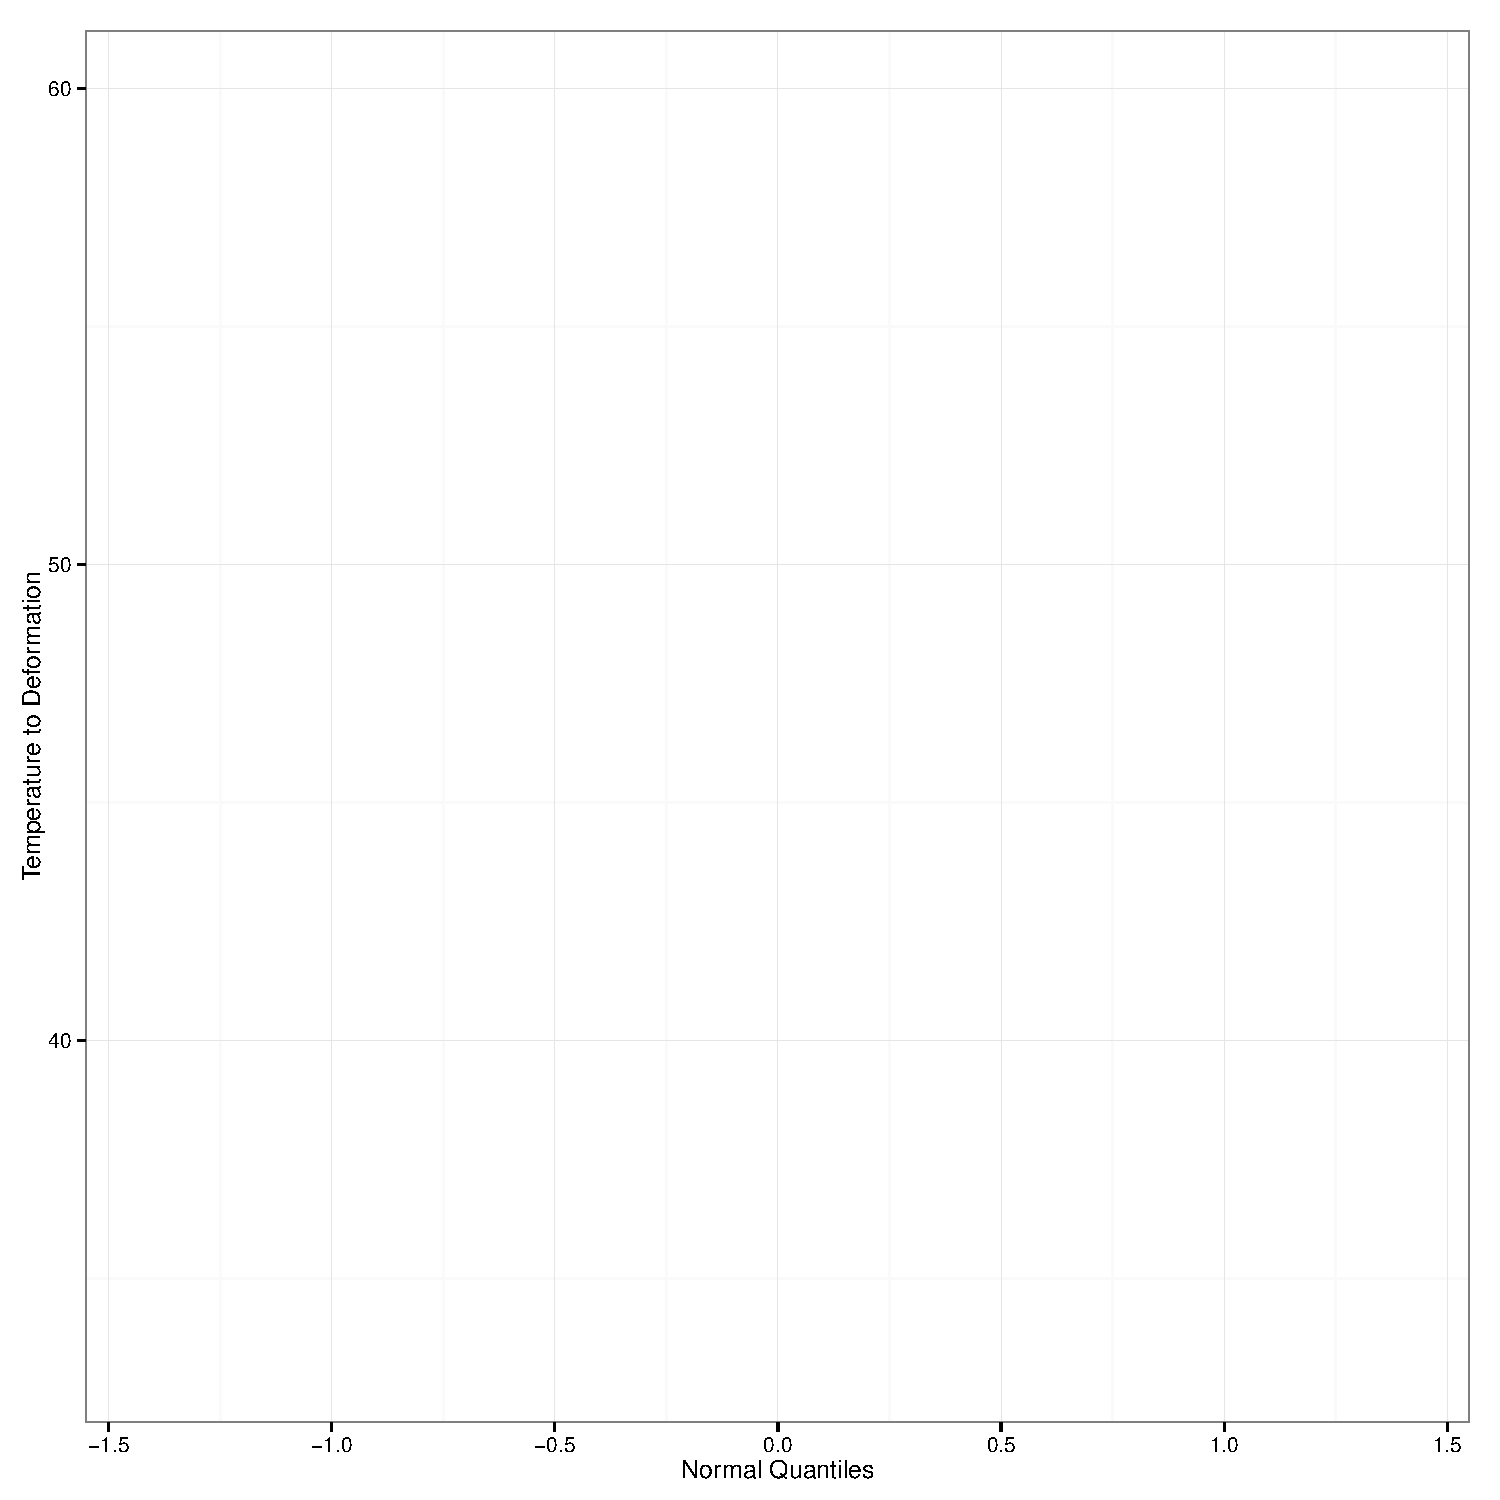
\includegraphics[width=.8\linewidth]{figure/unnamed-chunk-6-1} 

\end{knitrout}

\end{parts}
\pagebreak

\question

Professional engineers often encounter issues relating to \textit{human resources} as they advance in their careers
(building a better team of employees is after all not too different than improving any other system, at least on paper).
However, many of the "laws" governing human behavior are very different than the strict laws of physics.
For instance, a phenomenon known as the Dunning-Kruger effect states that for a given skill incompetent people will
\begin{itemize}
   \item fail to recognize their own lack of skill
   \item fail to recognize genuine skill in others
   \item fail to recognize the extremity of their inadequacy
   \item recognize and acknowledge their own lack of skill, after they are exposed to training for that skill
\end{itemize}

A group of 50 job applicants are asked to estimate their skill in technical writing. 
They are told they will be taking a test with a mean score of 50 and asked to guess what their score will be.
Then they are given the test and get an actual score. 

%-- : R code (Code in Document)


The results are depicted below (using the actual score on the x-axis):
\begin{center}
\begin{knitrout}
\definecolor{shadecolor}{rgb}{0.969, 0.969, 0.969}\color{fgcolor}
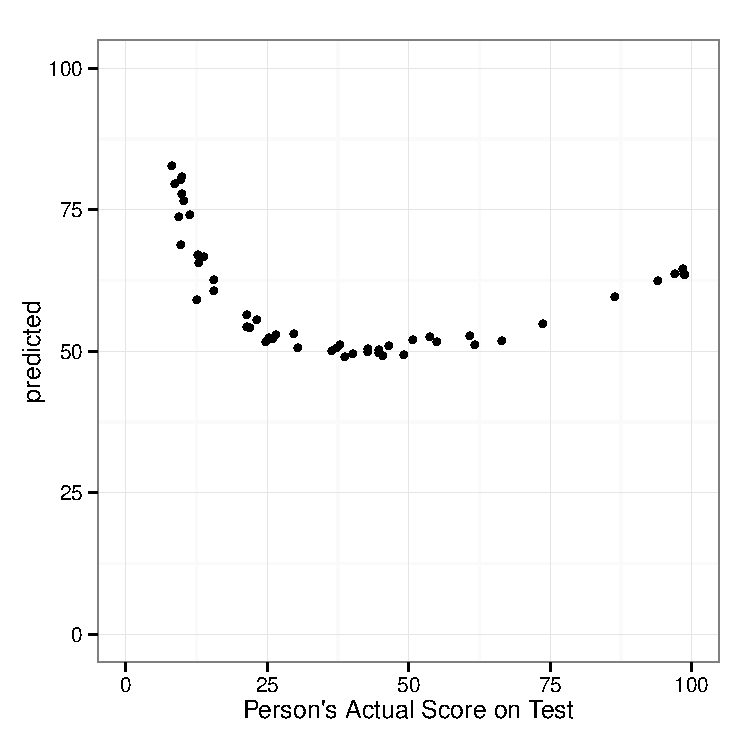
\includegraphics[width=.5\linewidth]{figure/unnamed-chunk-8-1} 

\end{knitrout}
\end{center}

Here are some summaries of the data (again using the actual score as the x-value and the person's evaluation of their score as the y-value):

$$
   \sum_{i=1}^{50} x_i = 1922 \hspace{3cm} \sum_{i=1}^{50} x_i^2 = 110659 \\
$$

$$
   \sum_{i=1}^{50} y_i = 2954 \hspace{3cm} \sum_{i=1}^{50} y_i^2 = 179606 \\
$$

$$
   \sum_{i=1}^{50} x_i y_i = 108893
$$

\begin{parts}
   \part Using the summaries above, fit a linear relationship between \textbf{the actual score} (x) and \textbf{the guessed score} (y). 
   \begin{subparts}
      \subpart[5] Write the equation of the fitted linear relationship. 
      \vspace{2cm}
      \subpart[5] Find and interpret the value of $R^2$ for the fitted linear relationship.
      \vspace{2cm}
      \subpart[5] Using the fitted line, what do we suppose a person will guess their score will be if they actually scored a 40.14.
      \vspace{2cm}
      \subpart[2] A person who scored a 40.14 on the test predicted that they would score 49.56. What is the residual for this person using the linear relationship?
      \vspace{2cm}
   \end{subparts}

   \newpage 

   \part The JMP output below comes from fitting a quadratic model using the actual score ("\verb!actual_score!") and the square of the actual score (\verb!actual_score^2!).

   \centerline{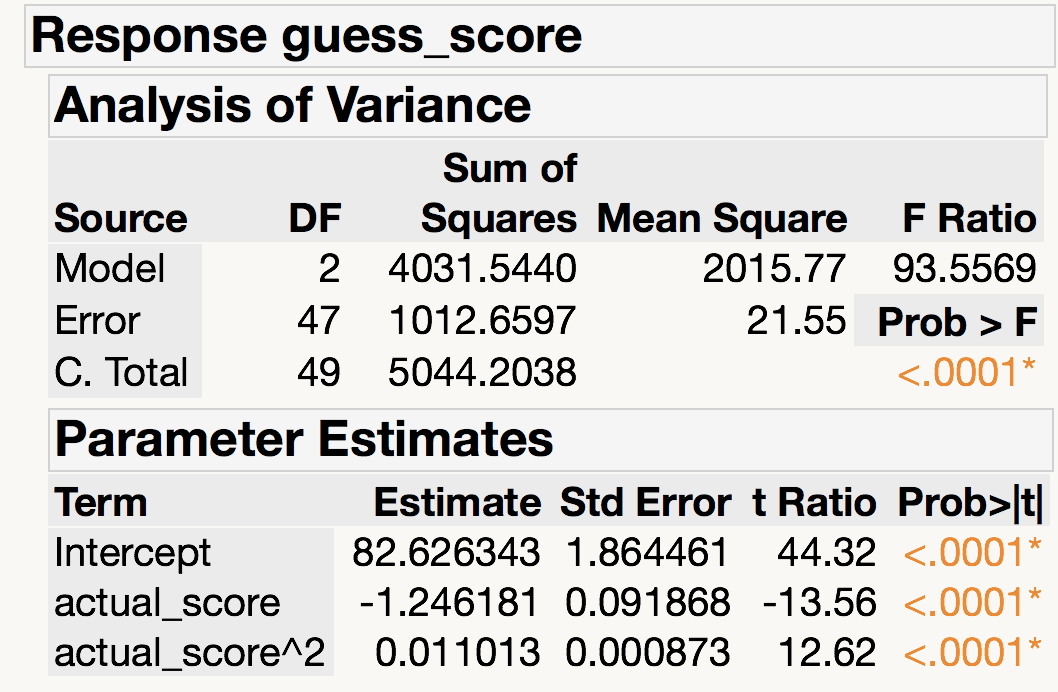
\includegraphics[scale=.2]{FitDK}}

   \begin{subparts}
      \subpart[5] Write the equation of the fitted quadratic relationship.
      \vspace{2cm}
      \subpart[5] Find and interpret the value of $R^2$ for the fitted quadratic relationship.
      \vspace{2cm}
      \subpart[5] Using the fitted quadratic relationship, what do we suppose a person will guess their score will be if they actually scored a 98.74.
      \vspace{2cm}
      \subpart[2] A person who scored a 98.74 on the test predicted that they would score 63.55. What is the residual for this person using the quadratic relationship?
      \vspace{2cm}
   \end{subparts}
\end{parts}

\end{questions}

\end{document}
